\documentclass{report}
\usepackage{graphicx}

\begin{document}

\title{Software Engineering\\CEN 4010 – U01\\Deliverable 2\\Blue Jay}
\date{\today}
\author{Team 3\and Mareo Yapp\and Brandon Lee\and Josselyn Ruiz\and Alex Collantes\and David Ramirez\and Professor Peter Clarke}
\maketitle

\begin{abstract}
There are many ways for people to communicate with others,
and social media is no exception. However,
many of the existing platforms provide limited security,
causing thousands of sensitive information to be leaked.
Even with existing forms of security in place,
the current methods vary from platform to platform,
with the most well-known social media sites generally having the weakest levels of encryption, or none.
BlueJay is a social platform for users to safely and securely post and share content over the internet using post sanitization,
SSL encryption, password encryption, and other forms of user security.
It takes the free-form posting of reddit and the social comforts of twitter to bring the same feeling of sharing content in a more secure setting.

This document will detail all the functional and non-functional requirements,
subsystems, and architectural and design patterns used to implement BlueJay.
The UML models displayed in the document were generated using StarUML.
The security protocols used to protect BlueJay include email verification,
forget password and login and out.
The architectural patterns in the package diagram were the three tier.
The major subsystem in the package diagram are Client, Logic and Database.
The design patterns used were the Template, Façade and Mediator.
\end{abstract}
 
\tableofcontents

\chapter{Introduction}
	This chapter will introduce the purpose of BlueJay (BJ),
	the functional and non-functional requirements of the use cases implemented.
	The software process model used will be identified along with the UML models that will be shown in the document.
\section{Purpose of system}
	Social media is a constant part of everyday life.
	People use it to stay in touch with their friends and family and to display their interests to the world,
	but far too often social media companies have been lapsing in protecting their users’ information.

	BlueJay (BJ) allows users to post text and images in a safe and secure manner to reduce the leaking of sensitive information,
	which can lead to fraud and identity theft.
	This will be done using many existing security techniques, such as password encryption, SSL encryption,
	and other safety measures that encourage users to prioritize securing their data.
\section{Requirements}
	\subsection{Functional requirements}
	These are the use cases we are implementing for the system.
	For more information, please see Appendix \ref{app:use_cases}
	\begin{enumerate}
		\item The system shall allow users to create an account
		\item The system shall allow users to create and upload posts
		\item The system shall allow users to reply to a post
		\item The system shall allow users to view posts on the site
		\item The system shall allow users to browse most recent popular post
		\item The system shall make users go through a process to access their account
		\item The system shall allow users to exit their accounts
		\item The system shall allow users to go through a process to access their account if they forget their password
		\item The system shall make users go through a process to get their password by answering 3 security questions
		\item The system shall send users an email asking them to verify their account
	\end{enumerate}
	\subsection{Non-functional requirements}
	Our system has many different non-functional requirements.
	\begin{description}
		\item [Usability] Users should be able to look at the page presented to them,
		and immediately recognize the functionality being exposed to them.
		\item [Reliability] The system will be highly available, up to 90\% of the time.
		And should be able to automatically recover from exceptional conditions.
		\item [Performance] The system will be highly responsive,
		except in the case of loading large posts.
	\end{description}


	Reliability: \\
		a.	All use cases have a consistent mean time to failure of 5 percent every 48 hours.\\
		b.	Some use cases should only allow for failure during a system maintenance (see use cases BJ021 - Login, BJ022 - Log out, BJS006 - Security Questions and BJS007 - Email Verification in Appendix B).\\
	Performance:\\ 
		a.	All use cases should have a maximum response time less than or equal to one second.\\
	Supportability: \\
		a.	All use case should be supported by browsers across multiple desktop and mobile devices.\\
	Frequency:\\
		a.	The average SM User will create and browse post around 30 times a day (see use cases BJ001 - Browse Post and BJ004 - Create Post in Appendix B).\\
		b.	The average SM User will view and reply to posts around 50 times a day (see use cases BJ002 - View Post and BJ006 - Reply to Post).\\
		c.	The average SM User will login and log out at most 15 times per day (see use cases BJ021 - Login and BJ022 - Log out in Appendix B).\\
		d.	Some use cases will only be used once (see use cases BJ015 - Account Creation, BJS005 - Forgot Password, BJS006 - Security Questions and BJS007 - Email Verification in Appendix B).\\
\section{Design methodology used} 
	The Unified Software Development Process model was used.
	The package, use case, deployment, ER, class, sequence and state machine diagram were used to represent the design.


\section{Definitions, acronyms, and abbreviations}
	Throughout the document, we use the following terms.
	\begin{description}
		\item [BlueJay] The name of our system, commonly abbreviated to BJ.
		\item [StarUML] Program we use to create models for our system.
		\item [SM User] A social media user, or for our system just a user.
		\item [HTML] Hyper-text markup language, the format we deliver content to our users in.
		\item [CSS] Cascading style sheets, file that determines how the HTML is rendered for clients.
		\item [SHA-256] Hashing algorithm we use to improve password security.
	\end{description}
\section{Overview of document}
	Chapter 2 will cover the software architecture such as the architectural patterns used.
	Chapter 3 will cover the diagrams used to represents the subsystems.
	Chapters 4 to 7 will be about the glossary, team signatures, references and appendices respectively.





\chapter{Proposed Software Architecture}
	This chapter will introduce the architectural patterns and detail the major subsystems used in the package diagram.
	Persistent data and the security protocols that were implemented will also be outlined.
\section{Overview}
	The primary architectural patter of our system is three-tier.
	As part of three-tier we have divided up the system into three main packages,
	client, logic, and database.
	The reason we chose three-tier over possibly four-tier or client-server,
	is because we don't need a special adapter layer between the client And
	the underlying business logic like four tier, but we do need a datastore
	unlike client-server.

	The secondary architectural pattern used in our system is repository.
	This secondary pattern exists, within the database package.
	The reason we chose repository

\section{Subsystem Decomposition}
\section{Hardware and Software Mapping}
\section{Persistent Data Management}
\section{Security Management}
BlueJay prides itself on its security, to ensure this various security protocols were implemented to protect unauthorized access to SM user’s accounts. These protocols include email verification, security questions and password recovery. With email verification when a SM user creates an account, they must provide an validate email address that is not being used by another account to activate their account. To access their account a user must log into by providing their username and password. In the off chance that user forgets their password they will be able to recover and change their old password by answering two questions they had previously set up and will have end when an email is sent to them.\\
\chapter{Detailed Design}
This chapter will introduce minimal class diagram for the subsystems and explain the purpose of each class. Along with the minimal class diagram this chapter will display the state machine and refined sequence diagrams. The design patterns used and the class sections that contain the OCL statements will be identified.\\
\section{Overview}
\section{State Machine}
\section{Object Interaction}
\section{Detailed Class Design}
The design patterns used were the Template, Façade and Mediator.\\
\chapter{Glossary}
BlueJay: BlueJay (BJ) is a social media platform that allows users to post texts and images in a safe and secure environment.\\
StarUML: StarUML is a software tool used to create UML diagrams.\\
SM User: Social media user; the user who is logged into the system.\\
MVC: Model View Controller is a software architectural pattern commonly used for developing user interfaces which divides the related program logic into three interconnected elements.\\
Three Tier: Three-tier architecture is a client-server software architecture pattern in which the user interface (presentation), functional process logic ("business rules"), computer data storage and data access are developed and maintained as independent modules, most often on separate platforms.\\
CSS: Cascading Style Sheets is a style sheet language used for describing the presentation of a document written in a markup language like HTML.\\
\chapter{Approval page with signatures of the team Appendix} 
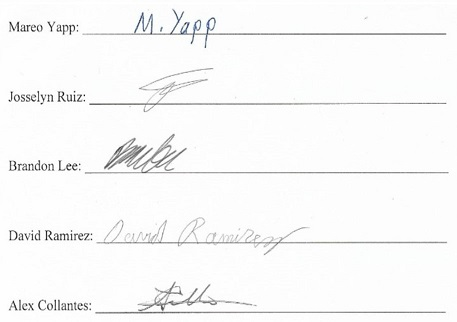
\includegraphics{Signatures}
\chapter{References}
\appendix
\section{Use Case Diagram}
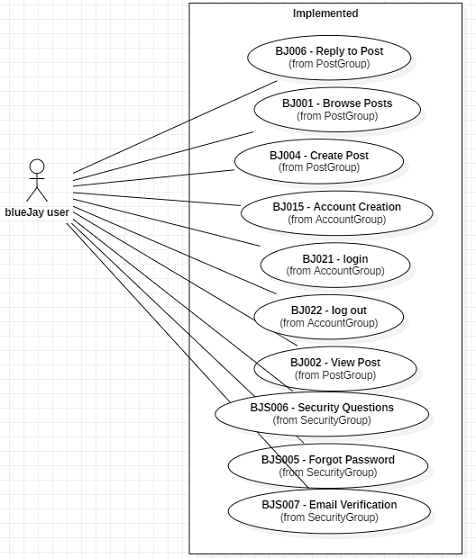
\includegraphics{UseCaseDiagram}
\section{Use Cases}
\label{app:use_cases}
Use Case ID: BJ001 – Browse Posts\\
Use Case Level: High-level\\
Details: The user requests that the homepage is to display all recently popular posts.\\
Actor: SM User\\
\\
Pre-conditions:\\
1.	User has access to the site.\\
\\
Description:\\
1.	User makes request to homepage.\\
a.	System queries database for most popular posts within the last 24 hours.\\
b.	Server constructs home page, showing most popular posts.\\
c.	Browser displays homepage.\\
\\
Post-conditions: \\
1.	Opening this page has no effect on the internal state of the server. The page is delivered to the client user.\\
\\
Alternative Courses of Action:\\
1.	In step (D1) the user has the option to search for specific posts.\\
2.	In step (D1) the user has the option to check his/her notifications.\\
\\
Exceptions: \\
1.	Posts could not be retrieved.\\
\\
Related Use Cases: \\
1.	BJ002 – View Post\\
2.	BJ003 – View Profile\\
\\
Decision Support\\
     Frequency: 30 times a day.\\
     Criticality: High. REASON\\
     Risk: Low. REASON\\
\\
Constraints:\\
1.	Usability\\
	a.	Average of 2 minutes for user to learn how to navigate pages and make posts\\
2.	Reliability\\
	a.	Mean time to failure - 5 percent every 48 hours is acceptable.\\
3.	Performance\\
	a.	Posts should load within two milliseconds.\\
4.	Supportability\\
	a.	Supported by browsers across multiple desktop and mobile devices.\\
\\
Modification History\\
     Owner: David Ramirez\\
     Initiation date: 8/27/2019\\
     Date last modified: 9/13/2019\\
\\
Use Case ID: BJ002 – View Post\\
Use Case Level: High-level\\
Details: User opens a post from the home page.\\
Actor: SM User\\
\\
Pre-conditions:\\
1.	User has access to the site.\\
\\
Description: \\
1. User selects a post on the page while searching through the posts, or within any of the extensions of that functionality.\\
a.	The browser requests the page with the selected post.\\
b.	The post, and all posts replying to that post are queried from the database.\\
c.	The server constructs the page to display the posts.\\
d.	The browser displays the page to the user.\\
\\
Post-conditions: \\
1.	Number of views on the post increases by one.\\
\\
Exceptions: \\
1.	Post could not be retrieved.\\
\\
Related Use Cases: \\
1.	BJ001 – Browse Post\\
\\
Decision Support\\
     Frequency: 50 times per day.\\
     Criticality: High. REASON\\
     Risk: Low. REASON\\
\\
Constraints:\\
1.	Usability\\
	a.	Average of 2 minutes for user to learn how to navigate pages and make posts\\
2.	Reliability\\
	a.	Mean time to failure - 5 percent every 48 hours is acceptable.\\
3.	Performance\\
	a.	Posts should be opened within five milliseconds.\\
4.	Supportability\\
	a.	Supported by browsers across multiple desktop and mobile devices.\\
\\
Modification History\\
     Owner: David Ramirez\\
     Initiation date: 8/27/2019\\
     Date last modified: 9/13/2019\\
\\
Use Case ID: BJ004 – Create Post\\
Use Case Level: High-level\\
Details: User creates a post and uploads it to make it publicly accessible.\\
Actor: SM User\\
\\
Pre-conditions: \\
1.	User has access to the site.\\
2.	User has an existing profile.\\
3.	User is logged into the site.\\
\\
Description: \\
1.	User clicks on the “Create Post” button found below their account snapshot on the righthand side of the home page.\\
	a.	Page reloads, showing the create post template. \\
2.	User enters desired text in provided text box\\
3.	User submits the form by selecting “Submit”\\
	a.	Submitted text is sanitized of all html tags, then saved to the database\\
4.	Use case ends when user is redirected to the page containing the newly submitted post\\
\\
Post-conditions: \\
1.	New post saved to database.\\
2.	Number of posts created for that user increases by one.\\
\\
Alternative Courses of Action:\\
1.	In step (D3) the user has the option to cancel the post creation before uploading the post.\\
\\
Extensions:\\
1.	BJ006 - Reply to Post\\
\\
Exceptions: \\
1.	User’s post could not be uploaded due to system downtime.\\
2.	User’s post could not be uploaded due to session timeout.\\
\\
Related Use Cases: \\
1.	BJ001 - Browse Posts\\
2.	BJ002 - View Posts\\
\\
Decision Support\\
     Frequency: 30 times per day.\\
     Criticality: High. REASON\\
     Risk: Medium. REASON\\
\\
Constraints: \\
1.	Usability\\
	a.	Average of 2 minutes for user to learn how to navigate pages and make posts\\
2.	Reliability\\
	a.	Mean time to failure - 5 percent every 48 hours is acceptable.\\
3.	Performance\\
	a.	Post form should open within five milliseconds.\\
4.	Supportability\\
	a.	Supported by browsers across multiple desktop and mobile devices.\\
\\
Modification History\\
     Owner: David Ramirez\\
     Initiation date: 8/27/2019\\
     Date last modified: 9/14/2019\\
\\
Use Case ID: BJ006 - Reply to Post\\
Use Case Level: High-level\\
Details: This use case walks through what the user does when they want to reply to a post.\\
Actor: SM User\\
\\
Pre-conditions: \\
1.	User has access to the site.\\
2.	User has an existing profile.\\
3.	User is logged into the site.\\
\\
Description: \\
1.	User clicks on a post they’re interested in. \\
	a.	The post pops up.\\
2.	User clicks on the reply icon. \\
	a.	A form opens with a text box to write a reply.\\
3.	User writes a reply and then clicks REPLY\\
	a.	The reply is displayed below the post   \\
\\
Post-conditions: \\
1.	Replies made by the user’s account will display at the top of the comment section when logged in as the user.\\
2.	The reply is stored as an extension of the post.\\
\\
Alternative Courses of Action:\\
1.	In step (D3) the user has the option to discard the reply.\\
\\
Exceptions: \\
1.	Page can time out after 5 minutes of inactivity.\\
\\
Related Use Cases: \\
1.	BJ001 – Browse Posts\\
2.	BJ002 – View Post\\
\\
Decision Support\\
     Frequency: 50 times per day.\\
     Criticality: High. Posting comments is one of the main uses of social media. \\
     Risk: Low. There is no real risk to this other than a scenario in which an unathorised user makes comments under the user’s account.\\
\\
Constraints:\\
1.	Usability\\
	a.	No training.\\
	b.	About 5 minutes to complete.\\
2.	Reliability\\
	a.	Mean time to failure - 5 percent every 48 hours is acceptable.\\
3.	Performance\\
	a.	Should take less than one second to display form.\\
4.	Supportability\\
a.	Supported by browsers across multiple desktop and mobile devices.\\
\\
Modification History\\
     Owner: Mareo Yapp\\
     Initiation date: 9/13/2019\\
     Date last modified: 9/14/2019\\
\\
Use Case ID: BJ015 – Account Creation\\
Use Case Level: High-level\\
Details: The user, being new to the system, creates a new account.\\
Actor: SM User\\
\\
Pre-conditions: \\
1.	User has no preexisting account.\\
2.	User types in “bluejay.com” and loads the system.\\
	a.	The system displays the log-in page.\\
\\
Description: \\
1.	User selects “New User” link. \\
	a.	The system displays a form requesting the following information\\
2.	User inputs his username and email, then selects “Continue”. \\
	a.	The system then asks for password following specific requirements.\\
3.	User inputs his/her wanted password and selects “Continue”. \\
	a.	The system loads the home page and a dialog box welcoming the user - “Welcome! Get ready to fly!”\\
\\
Post-conditions: \\
1.	Number of overall users increases by one.\\
2.	Number of posts made by the user is set to zero.\\
3.	Default image for user placed in his/her profile.\\
\\
Alternative Courses of Action:\\
1.	At any step the user has the option to cancel the creation of account by exiting the page.\\
\\
Related Use Cases: \\
1.	BJ001 – Browse Posts\\
2.	BJ002 – View Post\\
3.	BJ003 – View Profile\\
\\
Decision Support\\
     Frequency: An average user would only use this once.\\
     Criticality: High. REASON\\
     Risk: Medium. REASON\\
\\
Constraints:\\
1.	Usability\\
a.	No training needed.\\
2.	Reliability\\
a.	Mean time to failure - 5 percent every 48 hours is acceptable.\\
3.	Performance \\
a.	REASON\\
4.	Supportability\\
a.	Supported by browsers across multiple desktop and mobile devices.\\
\\
Modification History\\
     Owner: Josselyn Ruiz\\
     Initiation date: 8/27/2019\\
     Date last modified: 9/13/2019\\
\\
Use Case ID: BJ021 – Login\\
Use Case Level: High-level\\
Details:  The user types the website into the URL and is directed to the BlueJay website. The login page is then displayed, and the user is asked to input their username and password in order to gain access to the website.\\
Actor: SM User\\
\\
Pre-conditions: \\
1.	The user already has a Blue jay account.\\
\\
Description:\\
1.	The user enters the Blue jay URL\\
a.	System directes user to the login page.\\
2.	The user inputs their username and password into the blank fields.\\
3.	The user hits submit.\\
a.	Once the information is validated and correct, they gain access to the website.\\
\\
Trigger: \\
1.	The user logs onto the BlueJay website and is prompted to login.\\
2.	The system responds by taking the input and checking its validity.\\
\\
Post-conditions:\\
1.	The user now has access to the BlueJay website.\\
\\
Exceptions:\\
1.	The user has inputted the incorrect log in information.\\
\\
Decision Support\\
     Frequency: At most 15 times per day.\\
     Criticality: High. REASON\\
     Risk: High. REASON\\
     \\
Constraints: \\
1. Usability\\
a.	 No previous training needed. The user should be able to clearly understand the instructions on the screen.\\
2. Reliability\\
a.	Mean time to failure - 5 percent every 48 hours is acceptable.\\
b.	Only down time should be for system maintenance.\\
3. Performance\\
a.	Users should be able to log in within 1 second.\\
4. Supportability\\
a.	Supported by browsers across multiple desktop and mobile devices.\\
\\
Modification History\\
     Owner: Brandon Lee\\
     Initiation date: 8/27/2019\\
     Date last modified: 9/30/2019\\
\\
Use Case ID: BJ022 – Log Out\\
Use Case Level: High-level\\
Details:  The user navigates to their account. Then selects logout. The user is then signed out of their account.\\
Actor: SM User\\
\\
Pre-conditions: \\
1.	The user already has a Blue jay account\\
2.	The user is already logged in.\\
\\
Description: CONSISTENCY\\
1.	The user clicks on profile.\\
2.	The user selects log out of account.\\
3.	The user is logged out.\\
4.	Successful log out is displayed.\\
\\
Trigger: \\
1.	The user selects log out on their account.\\
2.	The system responds by logging the user out of their account.\\
\\
Post-conditions: \\
1.	The user is now logged out of their account.\\
\\
Exceptions: \\
1.	There has been an error logging out of the account.\\
\\
Related Use Cases: \\
1.	BJ022 – Login\\
2.	BJ002 – View Post\\
3.	BJ001 – Browse Post\\
\\
Decision Support\\
     Frequency: At most 15 times per day.\\
     Criticality: High. REASON\\
     Risk: High. REASON\\
\\
Constraints: \\
1.	Usability\\
a.	No previous training needed\\
2.  Reliability\\
a.	Mean time to failure - 5 percent every 48 hours is acceptable.\\
b.	Only down time should be for system maintenance.\\
3.	Performance\\
a.	Users should be able to complete logout in under 1 second.\\
4. 	Supportability\\
a. 	Supported by browsers across multiple desktop and mobile devices.\\
\\
Modification History\\
     Owner: Brandon Lee\\
     Initiation date: 8/27/2019\\
     Date last modified: 9/30/2019\\
\\
Use Case ID: BJS005 – Forgot Password\\
Use Case Level: High-level\\
Details: User attempts to restore his/her forgotten password by answering security questions.\\
Actor: SM User\\
\\
Pre-conditions: \\
1.	User has internet access\\
2.	User has an existing BlueJay profile\\
3.	User has attempted to log on, but the system shows password as incorrect\\
\\
Description: \\
1.	The user clicks on the ‘Forgot Password?’ link at the bottom of the login page. \\
	a.	The system responds by opening the forgot password page asking the user to answer 2 security questions.\\
2.	User answers first security question correctly\\
	a.	The system displays the next question\\
3.	User answers second security question correctly\\
	a.	The system displays the form to enter and re-enter a new password\\
4.	User enters a new password and selects “Confirm”\\
	a.	Use case ends by returning to the homepage of the site. \\
\\
Post-conditions: \\
1.	Password details for user updated.\\
\\
Alternative Courses of Action:\\
1.	At any step the user has the option to cancel resetting process.\\
2.	User attempts entering password and it is entered correctly.\\
\\
Decision Support\\
     Frequency: An average user should use this only once a day if they forget their password. \\
     Criticality: High. Users need to be able to login to their accounts.\\
     Risk: High. Someone with access to the users email address and background could not only change their password but also have complete access to their account.\\
\\
Constraints:\\
1.	Usability\\
	a.	No training needed.\\
	b.	Average of 2 minutes for user to complete.\\
2.	Reliability\\
	a.	Mean time to failure - 5 percent every 48 hours is acceptable.\\
3.	Performance\\
	a.	Should verify credentials in 5 milliseconds.\\
4.	Supportability\\
	a.	Supported by browsers across multiple desktop and mobile devices.\\
\\
Modification History\\
     Owner: Mareo Yapp\\
     Initiation date: 8/27/2019\\
     Date last modified: 9/13/2019\\
\\
Use Case ID: BJS006 – Security Questions\\
Use Case Level: High-level\\
Details:  In The event the user has forgotten their password, typed the incorrect password more than 3x, wish to change their password or any other means by which the user is attempting to recover their account, they will have to provide the correct answers to the 3 security questions that are associated with the account.\\
Actor: SM User\\
\\
Pre-conditions: \\
1.	The user has access to the internet.\\
2.	The user has been denied access to their account for one reason or another and needs to access their account.\\
\\
Description: INSUFFICENT\\
1.	The user has attempted to log into their account but has been denied access for one or several reasons such as:\\
a.	Incorrect password inputted 3x.\\
b.	Suspicious login.\\
c.	Wishes to change password.\\
2.	The system then asks the user to provide the answers to 3 security questions that are associated with the account.\\
a.	If correct then the user is granted access, if incorrect they are denied access.\\
\\
Post-conditions: \\
1.	Provided the answers to the security questions are correct, the user will have access to their account.\\
\\
Alternative Courses of Action:\\
1.	At any step the user has the option to cancel login.\\
\\
Extensions: \\
1.	BJ015 – Account Creation\\
\\
Decision Support\\
     Frequency: An average user should use this only once a day if they forget their password.\\
     Criticality: High. REASON\\
     Risk: High. REASON\\
\\
Constraints: \\
1.	Usability\\
a.	No previous training needed.\\
b.	Average of 2 minutes for user to complete.\\
2.	Reliability\\
a.	Mean time to failure - 5 percent every 48 hours is acceptable.\\
b.	Only down time should be for system maintenance.\\
3.	Performance\\
a.	Should verify in 5 milliseconds\\
4.	Supportability\\
a. 	Supported by browsers across multiple desktop and mobile devices.\\
\\
Modification History\\
     Owner: Brandon Lee\\
     Initiation date: 8/27/2019\\
     Date last modified: 9/14/2019\\
\\
Use Case ID: BJS007- Email Verification\\
Use Case Level: High-level\\
Details:  Once the user has finished inputting their credentials for their account, they will be asked to confirm their account via email confirmation.\\
Actor: SM User\\
\\
Pre-conditions: \\
1.	The user has already started the account creation process.\\
\\
Description: \\
1.	Server is adding new account to database.\\
2.	The system shall send a verification email to the email address of the new account.\\
3.	The user will click the link in their email to verify their account.\\
a.	Server marks the account as verified.\\
4.	Browser is redirected to homepage.\\
a.	Homepage is displayed to user.\\
\\
Post-conditions: INCOMPLETE \\
1.	Upon clicking \\
\\
Alternative Courses of Action:\\
1.	At any step the user has the option to cancel login.\\
\\
Extensions: \\
1.	BJ015 – Account Creation\\
\\
Decision Support\\
     Frequency: An average user would only use this once.\\
     Criticality: High. REASON\\
     Risk: High. REASON\\
\\
Constraints:\\
1.	Usability\\
	a.	No previous training needed. The user should be able to clearly understand the instructions on the screen.\\
	b.	Users should be able to complete questions in under 5 minutes.\\
2.	Reliability\\
\\	a.	Mean time to failure - 5 percent every 48 hours is acceptable.
\\	b.	Only down time should be for system maintenance.\\
3.	Performance\\
	a.	Should verify in 5 milliseconds.\\
4.	Supportability\\
	a.	Supported by browsers across multiple desktop and mobile devices.\\
\\
Modification History\\
     Owner: Brandon Lee\\
     Initiation date: 8/27/2019\\
     Date last modified: 9/14/2019\\
\section{Class Diagram}
\section{Class Interfaces}
\section{Meetings Diary}
ENTRY 1\\	
Location		ECS Lab\\
Starting Time		2:00pm\\
Duration		2 hours\\
Attendees		David, Brandon, Alex, Josselyn, Mareo\\
Late Attendees	Josselyn, Mareo\\
Absent		None\\
\\
Minutes Captured\\
-	Review class and sequence diagrams; to include java servlet\\
-	David went over class diagram\\
-	Use case implementation\\
o	Create Reply\\
o	Browse Post\\
o	Create Post\\
o	Log In\\
o	Log Out\\
o	View Post\\
o	Account Creation\\
o	Email Verification\\
o	Forgot Password\\
o	Security Questions (replaced Hide Password)\\
-	David and Alex to begin reviewing PHP and converting it to Java\\
-	Rewrite of cookies necessary\\
-	Roles Decided\\
o	David – Team Leader and Development\\
o	Josselyn – Minute Take and Developer\\
o	Brandon – Time Keeper and Quality Assurance\\
o	Alex – Developer and Requirements Engineer\\
o	Mareo – Requirements Engineer and Quality Assurance\\
\\
ENTRY 2\\	
Location		GL 166\\
Starting Time		5:50pm\\
Duration		25 minutes\\
Attendees		David, Alex, Josselyn, Mareo, Brandon\\
Late Attendees	None\\
Absent		None\\
\\
Minutes Captured\\
-	Mareo created a doc in Google docs; David suggests using Git Hub to create and edit document to minimize issues with formatting.\\
-	Alex suggests splitting up work in a more efficient way.\\
-	Databases already created during phase one. (Users and Posts)\\
-	Need to build ER diagram\\
-	Tasks to do\\
o	Pick two architectures to apply for project – prepare to present (three-tier, client/server, MVC)\\
o	PHP to Java conversion needed; Java DB revisit (Alex and David)\\
o	Document upload to Git Hub (Brandon, Mareo)\\
o	UI revisit (Josselyn)\\
o	Send initial diary entries (Josselyn)\\
\\
ENTRY 3\\	
Location		GL 166\\
Starting Time		6:00pm\\
Duration		20 minutes\\
Attendees		David, Alex, Josselyn, Mareo\\
Late Attendees	None\\
Absent		Brandon (out sick)\\
\\
Minutes Captured\\
-	David assisting Alex with Linux set up\\
-	Rough draft of deployment diagram made\\
-	Mareo aligning with GitHub documentation\\
-	Josselyn to find ER diagram programs that verifies if models are made correctly\\
-	Entities being included in ER Diagram\\
o	Profile\\
o	User\\
o	Post\\
\end{document}

\documentclass
